\clearpage
\newpage
\section{Segmentação Semântica}
\label{semantic:semantic}
\begin{itemize}
    \item citar \cite{Minaee2021}
    \item citar \cite{Arbelaez2012}
    \item citar \cite{Zhang2018}
\end{itemize}


\subsection{\textit{Fully Convolutional Networks} (FCN)}
\label{semantic:FCN}
Fully Conventional Networks são redes que trabalham com ... 
%%%%%%%%%%%%%%%%%%%%%%%%%%%%%%%%%%%%%%%%%%%%%%%%%%%%%%%%%%%%%%%%%%%%%%%%%%%%%%%%%%%%%%%%%%%%%%%%%%%%%
\begin{itemize}
    \item citar \cite{Shelhamer2016};
    \item citar \cite{Minaee2021}
\end{itemize}
%%%%%%%%%%%%%%%%%%%%%%%%%%%%%%%%%%%%%%%%%%%%%%%%%%%%%%%%%%%%%%%%%%%%%%%%%%%%%%%%%%%%%%%%%%%%%%%%%%%%%


\subsection{Métricas}

Tendo dito que o objetivo principal das segmentações semânticas está reacionado com o a assimilação de classes para cada um dos pixeis presentes na imagem \cite{Csurka} fazem-se necessárias métricas que mensurem o desenvolvimento positivo ou negativo do modelo em questão.

Sendo assim, nessa seção métricas comuns para o desenvolvimento de segmentações semânticas serão discutidos, sendo que dentre esses, são nomeadas as métricas baseadas em região (sessão \ref{semantic:pa}), F1 \textit{Score} (sessão \ref{semantic:f1}) e \textit{intersection over union} (sessão \ref{semantic:IoU}).


\subsubsection{\textit{Pixel Accuracy}}
\label{semantic:pa}

A métrica de \textit{pixel accuracy} (PA) é uma das métricas mais simples utilizadas no contexto de segmentação semântica, em que, na prática se resume na e razão entre o pixel classificado em relação ao total de pixeis na imagem \cite{Minaee2021}. Sendo assim, é possível expressar a sua formula pela equação \ref{semantic:eq:1}, sendo $K$ as classes presentes na imagem, independente se para um plano de fundo ou para primeiro plano, $p_{ij}$ para número de classes preditas($i$) pertencente a classe $j$.

\begin{equation}
    \label{semantic:eq:1}
    PA = \frac{\sum_{i=0}^{K} p_{ij}}{\sum_{i=0}^{K} \sum_{j=0}^{K} p_{ij}}
\end{equation}

Todavia, é relevante citar que essa métrica indicando apenas precisão dos pixeis, como o nome sugere e não é adequada para situações que há um desequilíbrio de classes (ou \textit{class imbalance}), situação em que determinadas classes dominam a cena e que se faz presente no mundo real.


\subsubsection{\textit{Intersection over Union} (IoU)}
\label{semantic:IoU}

Já a métrica de intersecção entre a união, do inglês \textit{Intersection over Union} (IoU) ou Jaccard Index, é uma métrica que não passa por problemas de \textit{class imbalance}, além de ser considerada uma das métricas mais comuns para esse tipo de atividade \cite{Minaee2021}.

Suas representação pode ser visualizada a partir da figura \ref{semantic:fig:1}, além de que pela equação \ref{semantic:eq:2} é possível entender que o resultado de IoU se dá pela divisão da intersecção da segmentação predita e \textit{ground truth}, pela união entre a segmentação predita e o \textit{ground truth}.

\begin{figure}[H]
    \centering
    \caption{Representação de IoU.}
    
\includegraphics[height=2.3in]{recursos/imagens/semantic/IoU.png}
    \label{semantic:fig:1}

    \vspace*{1 cm}
    Fonte: do próprio autor.
\end{figure}

\begin{equation}
    \label{semantic:eq:2}
    IoU = J(A,B) = \frac{|A \cap B|}{|A \cup B|}
\end{equation}

Após a criação dessa métrica, outras variações ganharam repercussão, das quais destaca-se \textbf{\textit{Mean Intersection-over-Union} (mIoU)}, a qual realiza a média entre todos os valores de IoU das classes presentes na cena e apresenta um valor escalar como resultado para a segmentação como um todo \cite{Minaee2021}, sendo utilizada em trabalhos como \cite{Mohan2020}.


\subsubsection{F1 \textit{Score}}
\label{semantic:f1}

Para a definição da métrica F1-\textit{score} que é extremamente comum na esfera de segmentação de imagens, é necessário ter ciência de antemão que ela é composta pelo uso de outras duas métricas, sendo elas: 1) precisão, que é a divisão de verdadeiros positivos pela soma de verdadeiros positivos e falsos positivos (expresso na equação \ref{semantic:eq:3}, assim como 2) revocação, que é a divisão de verdadeiros positivos pela soma de verdadeiros positivos e falsos negativos (expresso na equação \ref{semantic:eq:4}.

\begin{equation}
    \label{semantic:eq:3}
    \text{Precisão} = \frac{VP}{VP + FP}
\end{equation}

\begin{equation}
    \label{semantic:eq:4}
    \text{Revocação} = \frac{VP}{VP + FN}
\end{equation}

Assim, para a definição de F1-\textit{score} é utilizado a média harmônica entre a precisão e revocação \cite{Minaee2021}, a qual pode ser expressa pela equação \ref{semantic:eq:5}.

\begin{equation}
    \label{semantic:eq:5}
    F1-score = \frac{2 \text{Precisão} \text{Revocação}}{\text{Precisão} + \text{Revocação}}
\end{equation}

Por fim, vale comentar que para situações em que tem-se uma segmentação binária, o valor de F1-\textit{score} é semelhante ao valor do \textbf{coeficiente Dice}, o qual normalmente é utilizado para situações médicas \cite{Minaee2021} e utiliza conceitos de intersecção assim como a métrica de IoU (seção \ref{semantic:IoU}), visto que quando não está assimilado a situações binárias, pode ser representado pela equação \ref{semantic:eq:6} ou pela imagem \ref{semantic:fig:2}.

\begin{equation}
    \label{semantic:eq:6}
    Dice = \frac{2|A \cap B|}{|A| + |B|}
\end{equation}

\begin{figure}[H]
    \centering
    \caption{Representação do coeficiente Dice.}
    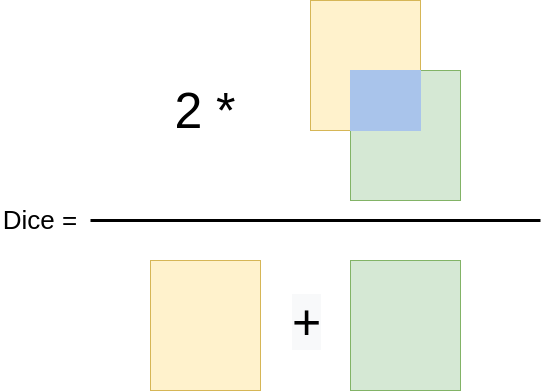
\includegraphics[height=2.3in]{recursos/imagens/semantic/dice.png}
    \label{semantic:fig:2}

    \vspace*{1 cm}
    Fonte: do próprio autor.
\end{figure}


\subsection{Considerações Finais da Seção}
\label{semantic:conclusion}

For example, for a pedestrian detection system, the whole body of person should belong to the same segment; how- ever, for an action recognition system, it might be necessary to segment different body parts into different classes. Other forms of image segmentation can focus on the most important object in a scene. A particular class of problem called saliency detection [14] is born from this. Other variants of this domain can be foreground-background separation problems. In many systems, such as im- age retrieval or visual question answering, it is often necessary to count the number of objects. Instance-specific segmentation addresses that issue.

%%%%%%%%%%%%%%%%%%%%%%%%%%%%%%%%%%%%%%%%%%%%%%%%%%%%%%%%%%%%%%%%%%%%%%%%%%%%%%%%%%%%%%%%%%%%%%%%%%%%%
\begin{itemize}
    \item falar dos problemas em tempo real \cite{Yu2018}
    \item falar dos problemas citados por \cite{Kirillov2019a}
\end{itemize}
%%%%%%%%%%%%%%%%%%%%%%%%%%%%%%%%%%%%%%%%%%%%%%%%%%%%%%%%%%%%%%%%%%%%%%%%%%%%%%%%%%%%%%%%%%%%%%%%%%%%%